\documentclass[tikz,border=5pt]{standalone}
\usepackage{pgfplots}
\usepgfplotslibrary{groupplots}
\pgfplotsset{compat=1.18}

\definecolor{corba}{HTML}{365FB3}
\definecolor{punt}{HTML}{B91C1C}
\definecolor{assimptota}{HTML}{6B7280}

\begin{document}
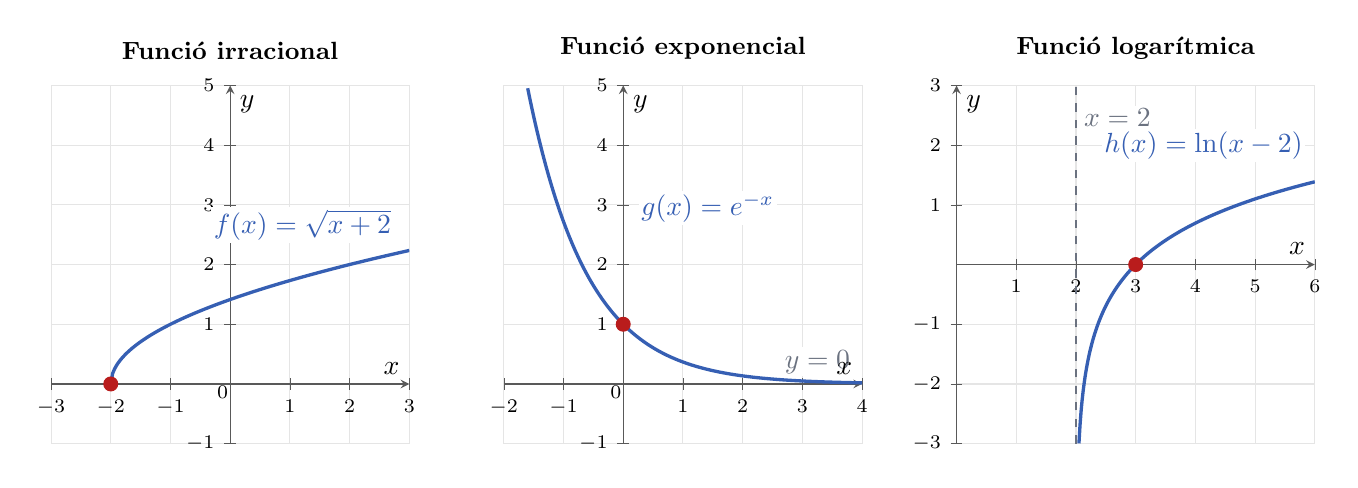
\begin{tikzpicture}
  \begin{groupplot}[
    group style={group size=3 by 1, horizontal sep=1.2cm},
    width=4.55cm,
    height=4.55cm,
    scale only axis,
    axis equal image,
    axis lines=middle,
    grid=major,
    grid style={black!10},
    axis line style={black!65},
    tick style={black!65},
    tick label style={font=\scriptsize},
    title style={font=\small\bfseries},
    xlabel={$x$},
    ylabel={$y$},
    clip=true,
  ]
    \nextgroupplot[
      title={Funció irracional},
      xmin=-3, xmax=3,
      ymin=-1, ymax=5,
      xtick={-3,-2,-1,0,1,2,3},
      ytick={-1,0,1,2,3,4,5},
    ]
      \addplot[corba, very thick, domain=-2:3, samples=160]
        {sqrt(x+2)};
      \addplot[only marks, mark=*, mark size=2.5pt, punt]
        coordinates {(-2,0)};
      \node[anchor=north east, font=\scriptsize, fill=white, inner sep=0.5pt]
        at (axis cs:0,0) {$0$};
      \node[anchor=south east, text=corba, fill=white, inner sep=1pt]
        at (axis cs:2.75,2.35) {$f(x)=\sqrt{x+2}$};

    \nextgroupplot[
      title={Funció exponencial},
      xmin=-2, xmax=4,
      ymin=-1, ymax=5,
      xtick={-2,-1,0,1,2,3,4},
      ytick={-1,0,1,2,3,4,5},
    ]
      \addplot[corba, very thick, domain=-1.6:4, samples=180]
        {exp(-x)};
      \addplot[only marks, mark=*, mark size=2.5pt, punt]
        coordinates {(0,1)};
      \node[anchor=north east, font=\scriptsize, fill=white, inner sep=0.5pt]
        at (axis cs:0,0) {$0$};
      \node[anchor=south west, text=assimptota, fill=white, inner sep=1pt]
        at (axis cs:2.65,0.12) {$y=0$};
      \node[anchor=south west, text=corba, fill=white, inner sep=1pt]
        at (axis cs:0.25,2.65) {$g(x)=e^{-x}$};

    \nextgroupplot[
      title={Funció logarítmica},
      xmin=0, xmax=6,
      ymin=-3, ymax=3,
      xtick={0,1,2,3,4,5,6},
      ytick={-3,-2,-1,0,1,2,3},
    ]
      \addplot[assimptota, dashed, thick]
        coordinates {(2,-3) (2,3)};
      \addplot[corba, very thick, domain=2.05:6, samples=220]
        {ln(x-2)};
      \addplot[only marks, mark=*, mark size=2.5pt, punt]
        coordinates {(3,0)};
      \node[anchor=north east, font=\scriptsize, fill=white, inner sep=0.5pt]
        at (axis cs:0,0) {$0$};
      \node[anchor=south west, text=assimptota, fill=white, inner sep=1pt]
        at (axis cs:2.08,2.25) {$x=2$};
      \node[anchor=south east, text=corba, fill=white, inner sep=1pt]
        at (axis cs:5.85,1.7) {$h(x)=\ln(x-2)$};
  \end{groupplot}
\end{tikzpicture}
\end{document}
